\chapter{Teil4}
\label{cha:Enthalpieübertrager}


\section{Enthalpieübertrager}
\label{sec:Enthalpieübertrager}

Der in dieser Untersuchung verwendete Enthalpieübertrager ist der ein Kreuzstromübertrager. Das heißt der Feedstrom und der Sweepstrom werden über Kreuz aneinander vorbei geführt. Ein klassischer Kreuzstromübertrager weißt einen quadratischen Querschnitt auf. Die Luftströme kreuzen sich in einem solche Übertrager daher in einem 90° Winkel. Im Gegensatz dazu weißt der hier verwendete Enthalpieübertrager einen sechseckigen Querschnitt auf, wie in Abbildung \ref{Geometrie Enthalpieuebertrager} dargestellt. Diese Geometrie führt dazu, dass die Luftströme in einem steileren Winkel aneinander vorbei Strömen. Daher ist anzunehmen, dass beim vorliegenden Enthalpieübertrager das Übertragungsverhalten leicht von dem eines reinen Kreuzstromübertragers abweichen und dass dieser teilweise Eigenschaften eines Gegenstromübertragers aufweist. 

\begin{figure} [h]
	\centering
	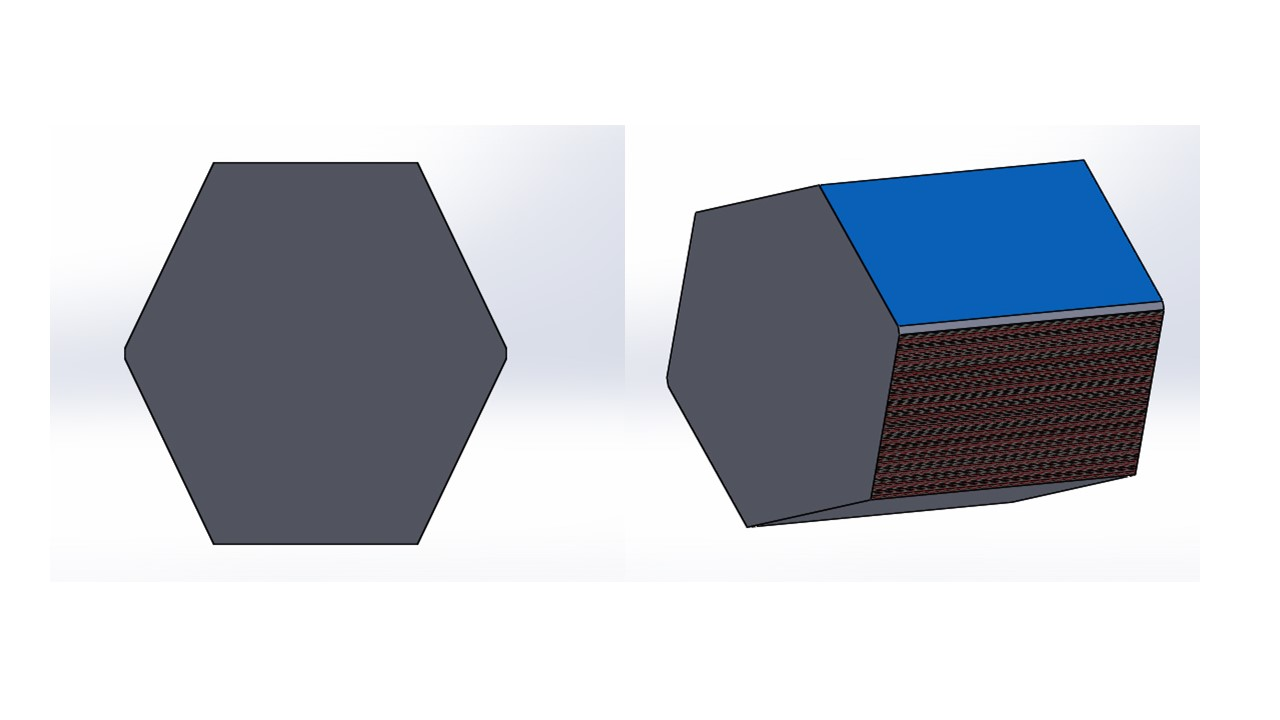
\includegraphics[width=0.98\textwidth]{pictures/Geometrie_Enthalpieuebertrager.jpg}
	\caption{Geometrie Enthalpieübertrager}
	\label{Geometrie Enthalpieuebertrager}
\end{figure}

Der Enthalpieübertrager hat eine Länge von 450 mm, eine Breite von 365 mm und ein Höhe von 365 mm. Die Anström- und Abströmflächen besitzen jeweils die Abmaße 450 x 196 mm. Der Abstand von der Anströmfläche einer Luftströmung zu ihrer Abströmfläche beträgt 333 mm. Die Übertragungsfläche jeder einzelnen Membran entspricht in etwa dem in Abbildung \ref{Geometrie Enthalpieuebertrager} dargestellten sechseckigen Querschnitt. Sie weißt jeweils eine Fläche von ca. 1030 cm² auf.   

Die Membranen des verwendeten Enthalpieübertragers bestehen aus Polyethylen und Polyether-Copolymer. Das Gehäuse und die Spacer aus Polystyrol. Es sind 185 Membranen mit einer Dicke von 0,11 mm und einem Abstand von 2,25 mm verbaut. Folglich weist der Enthalpieübertrager je 93 Strömungskanäle für den Sweepstrom und für den Feedstrom auf. 
 
 